\chapter{Learnersourcing Debugging and Design Hints}\label{chapter:classoverflow}

%Personalized support for students is a gold standard in education, but it scales poorly with the number of students. Prior work on \textit{learnersourcing} presented an approach for learners to engage in human computation tasks while trying to learn a new skill. Our key insight is that students, through their own experience struggling with a particular problem, can become experts on the particular optimizations they implement or bugs they resolve. These students can then generate hints for fellow students based on their new expertise. We present workflows that harvest and organize students' collective knowledge and advice for helping fellow novices through design problems in engineering. Systems embodying each workflow were evaluated in the context of a college-level computer architecture class with an enrollment of more than two hundred students each semester. We show that, given our design choices, students can create helpful hints for their peers that augment or even replace teachers' personalized assistance, when that assistance is not available.

%\section{Introduction}

One-on-one human tutoring is a costly gold standard in education. As established in Bloom's seminal work on tutoring, mastery-based instruction with corrective feedback can offer a substantial improvement in learning outcomes over conventional classroom teaching \cite{bloom19842}. However, personalized support does not scale well with the number of students enrolled. In large classes, it is often not feasible for students to get personalized hints from a teacher in a timely manner. Massive open online courses (MOOCs) can have even worse teacher-to-student ratios, by orders of magnitude. Intelligent tutoring systems have strived to simulate the type of personalized support received in one-on-one tutoring, but they are expensive and time-consuming to build. 

\begin{figure}
\centering
\includegraphics[width=0.75\columnwidth]{Body/figures/classoverflow/CombinedWorkflow_CameraReady.png}
\caption{In the \textit{self-reflection} workflow, students generate hints by reflecting on an obstacle they themselves have recently overcome. In the \textit{comparison} workflow, students compare their own solutions to those of other students, generating a hint as a byproduct of explaining how one might get from one solution to the other.}
\label{fig:workflow}
\end{figure}

In this chapter, learners are asked to generate personalized hints for each other. Prior work on \textit{learnersourcing} demonstrates how learners can collectively generate educational content for future learners, such as video outlines and exam questions, while engaging in a meaningful learning experience themselves \cite{kim2013learnersourcing,weir2015,mitros2015}. The proposed benefit of learnersourcing is that learners are not only more intrinsically motivated to engage with the learning content to begin with, but may also benefit pedagogically from the task itself.

This work builds upon learnersourcing by exploring how it can be applied to the generation of personalized hints during more complex problem solving. Whereas prior work determined which task to present to the learner depending on what information was still needed \cite{weir2015}, many educational topics like digital circuit design require more domain expertise, raising the question of which learners should be assigned to generate which hints. Beyond learnersourcing subgoals for how-to videos, this work takes on the challenge of generating content that is tailored to both the \textit{hint-receiver}'s current progress and the \textit{hint-author}'s likely level of understanding. 

This chapter describes two workflows for learnersourcing hints that assign hint-generating tasks to learners based on what problems the learner has recently solved. In the \textit{self-reflection} workflow, students generate hints by reflecting on an obstacle they themselves have recently overcome. In the \textit{comparison} workflow, students compare their own solutions to those of other students, generating a hint as a byproduct of explaining how one might get from one solution to the other. The second workflow can operate on the output of the first, as shown in Figure \ref{fig:workflow}. In both workflows, the key insight is that, through their own experience struggling with a particular problem, learners can become experts on the particular optimizations they implement and bugs they resolve. The workflows can take pressure off teaching staff while giving students the valuable educational experiences of reflection and generating explanations. 

While such workflows could have many applications, this paper presents a specific application within a college-level computer architecture class. In this course, students implement, debug, and optimize simulated processors by constructing digital circuits. During both the debugging and optimization process, hints are one mechanism for teachers to help students fix and optimize their circuits. This paper applies our learnersourcing workflows to two kinds of hints: \textit{debugging hints} and \textit{optimization hints}. A debugging hint is a student's attempt to help a future student change their solution so it generates the expected output for a particular input. An optimization hint is a student's attempt to help a future student get from one correct solution to another, more optimal solution. When hint-receivers encounter that particular situation during their problem-solving process, the hints can be shown to them as if they are the personalized hints an intelligent tutoring system might generate, or that a teacher might provide during a one-on-one interaction. 

\section{System Design}
There are a number of necessary decisions to make when designing interventions to collect and deliver hints:

{\it When should learners be asked to provide hints?} As soon as a student has resolved a bug, they may have some expertise about that bug that they can share with other students. If too much time has passed between resolving the bug and writing a hint, the student may forget necessary details and context, or forget the bug altogether. A previous learnersourcing system also prompted students to contribute content immediately after having experienced it themselves, for similar reasons \cite{weir2015}.

{\it How should learners access hints?} Hints can be distributed using either a \textit{push} or \textit{pull} model, and can involve displaying either \textit{all} or \textit{some} of the hints. For example, a push model might display hints as a constantly updating resource, whereas a pull model could dispense hints to individual students just-in-time, when a student needs help. The hints could be algorithmically selected based on the student's work so far and the hints they have already received. I explored both push and pull models, using the push-all model for distributing debugging hints and the pull-some model for distributing optimization hints. Generating optimization hints was a required reflection activity, so the volume and redundancy of these hints made a push-all model potentially overwhelming.

{\it What hints can I ask, or allow, a student to generate?} In cases where the student's \textit{start state} (prior to overcoming an obstacle) and \textit{end state} (after overcoming an obstacle) are known, such as when a student fixes a bug, the system can ask the student to create a hint helping other students encountering a similar bug or start state. For example, in the case of circuit design, I consider a student who has recently fixed a bug resolving a particular verification error to be capable of writing a debugging hint associated with that verification error.

In many cases, however, a student might not face any explicit obstacle, or their start state may not be known. For example, a student might naturally arrive at a highly optimal circuit design without having first tried a less optimal design. Regardless of the path to their solution, the student could generate hints by comparing their own solution to a more optimal solution, or to a less optimal solution. In this chapter, I explore both of these directions by asking each student to do both comparisons. To keep hint generation relevant to the learner's current task and to minimize cognitive load, I did not ask students to generate hints between pairs of solutions when they were familiar with neither solution.

{\it How should hints be indexed?} Indexing hints by a meaningful feature of student solutions allows students to more easily find relevant hints in a push model of hint distribution and allows the system to deliver more relevant hints to each student in a pull model of hint distribution. Optimization hints could be indexed by the learner's start state, end state, or both with respect to performance. Debugging hints could be indexed by verification errors. 

During debugging, students' solutions are run through sequences of teacher-designed test inputs. A {\it verification error} occurs when a student's solution does not return the expected values. Because test cases have a specification of actual and expected outputs for each input, I decided to index debugging hints by the tests for which the solution deviates from the expected output. In other words, debugging hints are associated with the verification error that disappears if the bug is resolved. 

During optimization, the goal is not simply to attain a correct solution, but rather to arrive at a more optimal correct solution. I decided to index optimization hints by both start and end states: the leap from a less optimal solution to a more optimal solution that the hint is intended to inspire. These states, the solutions themselves, are complex circuit objects; I use the number of transistors in a solution as a metric of its optimality. In this indexing scheme, all hints written with the intent of helping a student with a 114-transistor solution create a 96-transistor solution are binned together.

{\it Which hints should a student receive?} In the push-all model of hint distribution, this question is not relevant, but in the pull-some model of hint distribution, it may be critical. Ideally, students would receive a progression of increasingly specific hints, following patterns of adaptive scaffolding established in intelligent tutoring system literature \cite{andes}, helping them reach a more correct or optimal solution on the spectrum. 

This ideal still leaves room for design choices about exactly which hints to deliver in a pull model of distribution. For example, during the optimization stage of a student's assignment, the system could \textit{always} give the student hints that help them create the \textit{next optimal solution} found by other students (see Figure \ref{fig:sankey}). This would hopefully be an optimization challenge that falls within the student's zone of proximal development \cite{ZMP}. However, this may be too cautious. If a student's solution is far less optimal than the \textit{most common solution}, then the system could give the student hints to help them leap directly to that most common solution, without first creating any intermediate solutions. This strategy ignores how large a leap outside their zone of proximal development this might be, but it ensures that the student is exposed to the ideas, presented in those hints, that are necessary for implementing a solution at least as optimal as the most common one. I chose this latter option, both hinting students toward the most common solution and hinting students with the most common solution toward the most optimal solution.

\begin{figure}
\centering
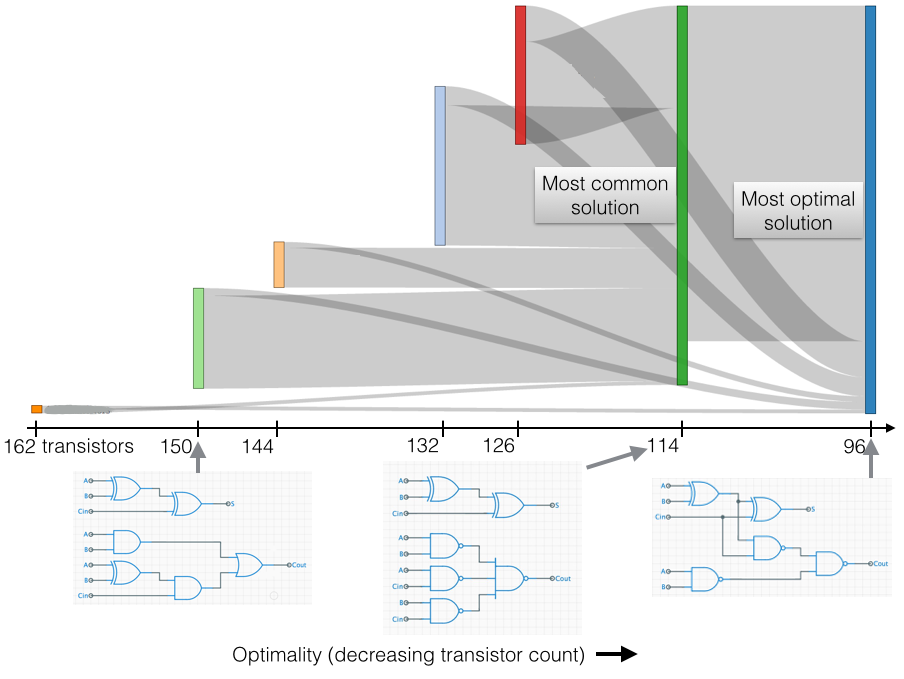
\includegraphics[width=1.0\columnwidth]{Body/figures/classoverflow/annotated_Sankey_onecolumn.png}
\caption{Sankey diagram of hints composed between types of correct solutions, binned by the number of transistors they contain. The optimal solution has only 21 gates and 96 transistors while the most common solution generated by students has 24 gates and 114 transistors.}
\label{fig:sankey}
\end{figure}

{\it Should hint creation be a required task?} As discussed in Related Work, generating hints can be a valuable part of the learning process. I required all students to generate optimization hints as part of a reflection activity immediately after submitting their first correct circuit. I did not require students to generate debugging hints. This is because the number of bugs encountered could be large, and unlike optimizations, many bugs also may not lead to significant conceptual gain upon reflection. Because debugging hints are immediately pushed out to all students, I keep both hint creation and upvotes voluntary to minimize the signal-to-noise ratio in hint quality.

{\it How should the variation in hint quality be handled?} In the push model of hint distribution, I used users' upvotes to sort hints by quality. In the pull model of hint distribution, I took advantage of the redundancy of the hints, and presented five hints at once. If one or more redundant hints were of poor quality, their aggregate message might still be helpful for a student. If most of the hints were about a feature that is irrelevant to the student receiving the hints, the remaining hint(s) might be about something different and more relevant. I limited each set of hints to a size of five to avoid overwhelming the learner with too many hints.

{\it How public should the hint-author be?} Many systems for question-answering have a reputation system, where the author is known and recognized for contributing answers. Previous work at CSCW has examined whether reputation would improve class forum participation \cite{reputation}. For simplicity, I chose to leave student identities hidden.

{\bf Final Workflows} In the self-reflection workflow, students iteratively modify their solutions to pass as many teacher-created tests as possible. For any verification error revealed by those tests, students can look up hints for what modifications might cause their solution to pass that test case instead. The hints are stored in a database indexed by the verification errors they are intended to address. When students fix a bug in their own solution, they can reflect on their fix and contribute a hint to the database for others struggling with the same verification error. The self-reflection step turns a successful bug fix into a shareable hint. It is effectively a self-explanation exercise, since the hint is not a conversation starter; it is meant to stand alone for any future student to consult. As studied in prior work \cite{selfexplanation}, self-explanation helps students integrate new information into existing knowledge.

In the comparison workflow, students compare their correct solution to alternative correct solutions previously submitted by other students or teachers. They are prompted to compare their solution to a solution \textit{W} with worse performance and generate an optimization hint for students who have solutions like \textit{W}. They are then prompted to compare their solution to a solution \textit{B} with better performance and generate an optimization hint for students who have solutions like their own, which are not yet as performant as solutions like \textit{B}. In each case, the student is generating an optimization hint to help students increase the performance of their solutions. Students who receive these hints use them as guidance while optimizing their own solutions. Figure \ref{fig:workflow} illustrates both workflows.

\section{User Interfaces} 
I designed two user interfaces, one for each workflow. To learnersource debugging hints with the self-reflection workflow, my co-authors and I built and deployed {\it Dear Beta}, a Meteor web application that serves as a central repository of debugging advice for and by students in the class. The name alludes to both the ``Dear Abby'' advice column and the Beta processor that students create in the class. To learnersource optimization hints with the comparison workflow, I designed {\it Dear Gamma}, a web interface students were required to fill out as a reflection activity after submitting their final correct circuit for a class assignment.

\subsection{Dear Beta}

I applied the self-reflection workflow to processor debugging. Consider students working on their Beta processors within the digital circuit development environment provided by the computer architecture class. Students run a staff-designed test file {\it x} on their circuit. The development environment alerts them to a verification error: for a particular input (test number {\it n}), {\it y} was the expected output and the student's circuit returned {\it z}. 

Students eliminate verification errors by fixing bugs in their circuits. They may use trial and error, methodically examine internal simulated voltages, or experience a flash of insight. On the Dear Beta website, they can post a hint for others derived from their insight and indexed by the verification error it caused. In the process of creating a hint, students have a chance to reflect on their own process of resolving the error.  Other students encountering that verification error can look up these hints, upvote helpful hints, and contribute new hints. Hints for each error are sorted by the number of upvotes they receive.

After further examining their malfunctioning processor with no success, some students may open the Dear Beta website in order to get help (Figure \ref{fig:hints}). Dear Beta displays all errors and hints, sorted by test file name {\it x}, then test number {\it n}. The student can either scroll to find hints for their verification error or jump directly to them by entering {\it x} and {\it n} into the bar pinned to the top of the page. If the error was not yet in the Dear Beta system, the error will be added and scrolled into view. 

If there are no hints yet, or if the hints are unhelpful, the student can click the ``Request'' button to the left of the error, which increments a counter. This button helps communicate the need for hints for a particular verification error to potential hint writers. This is analogous to the ``Want Answers'' button and counter on Quora, a popular question-and-answer site. 

If the student resolves their verification error and feels that the existing hints were insufficient or incomplete, they can click in the text box labeled ``Add a hint!'' so that it expands into a larger textbox sufficient for typing out a paragraph of their own hint text (Figure \ref{fig:contrib}). Their new hint may be a clearer rephrase of an existing hint or hint at yet another way to resolve the verification error. Given the variety of processor designs and implementations, there may be several ways any given verification error may be thrown. 

\begin{figure}
\centering
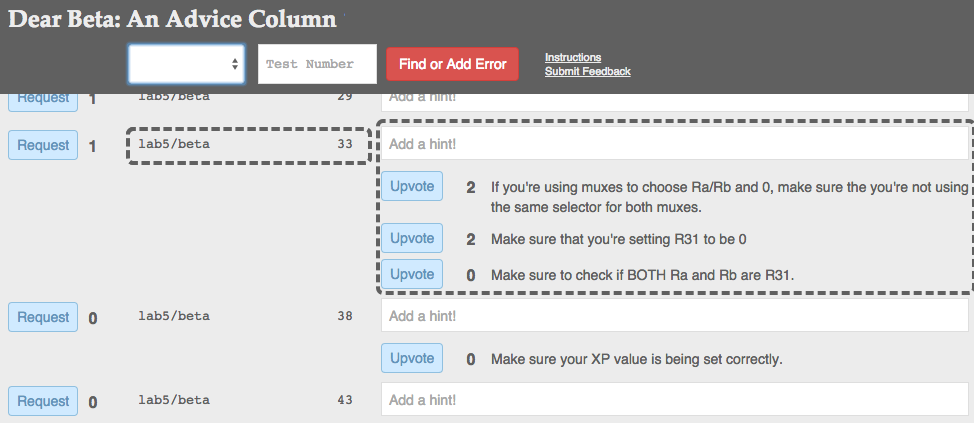
\includegraphics[width=1.0\columnwidth]{Body/figures/classoverflow/hints_modified.png}
\caption{{\it Dear Beta} serves as a central repository of debugging advice for and by students, indexed by verification errors. In this figure, there are three learnersourced hints, sorted by upvotes, for a verification error on test no. 33 in the `lab5/beta' checkoff file.}
\label{fig:hints}

\bigskip
\centering
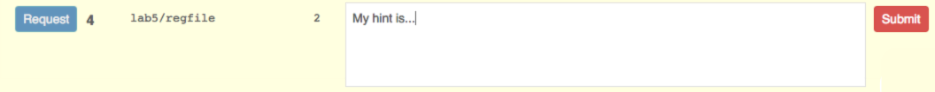
\includegraphics[width=1.0\columnwidth]{Body/figures/classoverflow/contrib_shortened.png}
\caption{After fixing a bug, students can add a hint for others, addressing what mistake prevented their own solution from passing this particular verification test.}
\label{fig:contrib}
\end{figure}

\subsubsection{Teacher Feedback on Early Prototypes of Dear Beta}

\todo{finish removing we's}

After deploying initial prototypes of Dear Beta for two semesters, we invited Teaching Assistants to share their complaints, requests, and experiences with us. Four TAs were interviewed, in person or by email, and their feedback and experiences informed Dear Beta's final design.

Both $TA_{1}$ and $TA_{3}$ adapted to Dear Beta's deployment by first asking each help-seeking student if they had already consulted Dear Beta. If they had not, $TA_{1}$ came back to them after visiting everyone else in the lab help queue. By then, they had often already resolved their problem with Dear Beta's hints, and had a new bug they wanted help debugging. 

Dear Beta was used as a debugging aid for both students and teachers. $TA_{2}$ described Dear Beta as a ``starting point'' for students, many of whom used it diligently during debugging. $TA_{2}$ appreciated that students who did ask for her help no longer said, ``My Beta isn't working. Tell me why.'' Instead, they used Dear Beta as a starting point, to help them identify potential locations of a bug in many pages of code. Not just helpful for students, $TA_{3}$ was able to describe with specific examples how Dear Beta \textit{helped him} help students quickly resolve common bugs.

$TA_{2}$ wondered if the extra hints were making it too easy to complete the lab, possibly letting students pass without understanding. $TA_{3}$ echoed this concern, but he made sure each student actually understood the Dear Beta hints whenever he personally guided them through the debugging process.

TAs identified both strengths and weakness in Dear Beta's design. $TA_{1}$ strongly supported Dear Beta's existing design as a single scannable sorted list for quickly finding hints, rather than a purely search-based hint retrieval mechanism or the more general class forum. However, the affordances for contributing new hints in the initial prototype were not obvious and rarely visible on small screens. As a result, $TA_{2}$ was concerned that the level of student involvement in producing hints might be too low. The final Dear Beta design is more externally consistent with other participatory Q\&A systems, has more salient buttons for contributing new hints, and a responsive design that accommodates screens as small as that of a cell phone. 

$TA_{4}$ was absent during most of Dear Beta's deployment but still regularly recommended Dear Beta to students who asked for her help over email. A fifth TA declined to be interviewed; she felt that she had not interacted with Dear Beta enough.

\subsection{Dear Gamma}

In order to learnersource optimization hints, we caught students at a different stage in their learning process: right after they passed all verification tests for a particular digital circuit, the Full Adder. Because students may have arrived at their solution without encountering any particular optimization obstacles, Dear Gamma uses the comparison workflow for learnersourcing rather than the self-reflection workflow. 

The comparison workflow is modified slightly, to accommodate the requirements of the course lecturer, who wanted to make sure that all students get a chance to consider both the most common and the most optimal solutions. The collection of previous student solutions in Figure \ref{fig:workflow} was also curated by the lecturer. If a student's solution is larger than the most common solution, they are not shown solutions larger than their own; instead, they are asked to consider both the most common and the most optimal solutions, so they benefit from seeing both without doing extra work overall. Students with the most optimal solution only consider alternative solutions that are worse than theirs. Figure \ref{fig:deargamma} shows an example of the page for a student with a 114-transistor solution.

In this activity, students are given a pair of solutions and asked to give a hint to future students about how to improve from the less optimal solution to the more optimal solution. Students write hints for two such pairs of solutions. In each pair, one of the solutions is always their own. When the student's own solution is the better solution in the pair, then the student can hint at what the peer might have missed. For example, {\it Remember DeMorgan's Law: you could replace the `OR' of `ANDs' with a `NAND' of `NANDs.'} When the students' own solution is the poorer solution in the pair, they are challenged to first understand how the better solution uses fewer transistors, and then write a hint about the insight for a peer. To aid the student in comparing solutions, the Dear Gamma interface displays the student's own solution as a reminder of their design, as well as an alternative picked from among other students' solutions.

Specifically, if a student's solution {\it S} is just as or more optimal than the most common solution, they are asked to (1) write a hint to help a future student with a less optimal solution reach solution {\it S} and (2) write a hint to help a student with solution {\it S} reach the most optimal solution. If a student's solution {\it S} is less optimal than the most common solution, they are asked to write a hint to help a student with solution {\it S} reach (1) the most common solution and (2) the most optimal solution. This scheme ensures that all students are familiar with the most common solution and the most optimal solution and have written two hints to help future students improve the optimality of their solutions. 

\begin{figure}
\centering
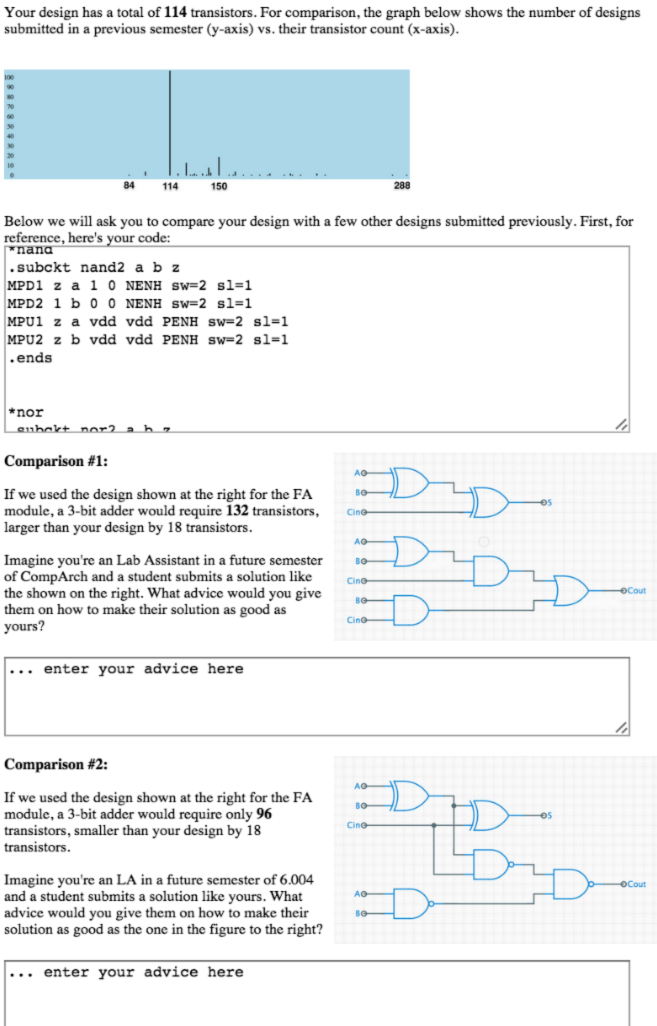
\includegraphics[width=0.70\columnwidth]{Body/figures/classoverflow/deargamma_shortened.png}
\caption{This is the Dear Gamma interface for a student with a solution containing 114 transistors. In the first comparison, they are asked to write a hint for a future student with a larger (less optimal) correct solution. In the second comparison, they are asked to write a hint for a future student with a solution similar to their own so that they may reach the smallest (most optimal) correct solution.}
\label{fig:deargamma}
\end{figure}

\section{Evaluation}

To evaluate the extent to which learnersourced hints can support problem solving, we deployed Dear Beta and Dear Gamma to the computer architecture class, which had an enrollment of more than two hundred students. Dear Beta was deployed for 6 weeks, during which we collected student-generated debugging hints and observed the simultaneous usage of those hints in a real-world setting. Dear Gamma's optimization hint collection interface was released to students as part of a particular lab. We then conducted a lab study with nine students to understand how they solve a typical engineering problem using these learnersourced optimization hints. 

The questions our evaluation sought to answer are: (1) {\it What are the characteristics of student-generated hints?} and (2) {\it Can learners solve problems using those hints?}

\section{Dear Beta}
The Dear Beta website was released as a stand-alone additional resource for students one week prior to the due date for the final circuit design lab. Students were made aware of its existence through a class forum announcement and signs on chalkboards in the course's computer lab. It was left up for the remainder of the semester for students to refer to, if completing work late. We tracked student logins and engagement with the site's features. An initial prototype of Dear Beta was deployed for two consecutive semesters prior to this final system design and study, as well.

\section{Dear Gamma}

\subsubsection{Hint Succession and Categorization}
While Dear Beta makes all hints available at all times, Dear Gamma is modeled on the hint-giving mechanism of an intelligent tutoring system. In prior work, sequences of hints have been posited to facilitate learning due to their similarity with sequences used in expert human tutoring, as well as their support of human memory processes \cite{sottilare2014design}. Therefore, we further decomposed the hints collected with Dear Gamma into the three kinds of hints that typically comprise a hint sequence: 1) \textit{pointing hints} direct the student's attention to the location of error in case the student understood the general principle but did not know to apply it; 2) \textit{teaching hints} explain why a better solution exists by stating the relevant principle or concept; 3) \textit{bottom-out hints} indicate concretely what the student should do \cite{andes}. 

Two researchers independently categorized the 435 collected Dear Gamma hints into six different categories: pure pointing hints ($p$), pointing and teaching hints ($pt$), pure teaching hints ($t$), teaching and bottom-out hints ($tb$), pure bottom-out hints ($b$), and hints that are irrelevant or clearly not helpful. They first independently labeled the first 30 hints. After discussing disagreements and iterating on their understanding of the hint categories, the coders then categorized the remaining 405 hints. 

If one coder labeled a hint as a hybrid between two categories (i.e., teaching and pointing) while the other coder labeled it with only one category (i.e., pointing), we assigned the hint to the pure category (i.e., pointing) that was in common between the two coders' labels. If there was no shared category across the two coders, the hint was discarded. We also excluded the minority of hints (3.2\%) that were labeled as irrelevant or unhelpful.

\subsubsection{Lab Study}

Nine out of the 226 current students in the computer architecture course participated in the study. These students were recruited through a course forum post. Participants were given \$30 for the study, which lasted one hour. We informed students that we were studying the effectiveness of hints for optimizing circuits so that they use fewer transistors.

During the study, we presented the hints as anonymous, potentially helpful messages. Three batches of hints were shown in the order of pointing, teaching, and bottom-out, but randomly selected within each category. Students began by opening up their previously completed lab and reviewing their solution. The experimenter noted down the number of transistors in their solution, and randomly selected five pointing-type hints for a solution of that size from the Dear Gamma collection. For example, if the student had 114 transistors in their solution, they received five hints previously generated by students who had written a hint to help improve a 114-transistor solution. Because hints may be of variable quality, the researcher presented hints in batches of five to increase the chances that one of them might be helpful.

The experimenter then asked the student to reduce the number of transistors in their solution. The experimenter explained that there were two more batches of five hints ready for them if they became stuck. These two batches were teaching hints and bottom-out hints. Students could consult outside resources like the course website and Google as well. 

After receiving each batch of hints, participants answered the following 7-point Likert-scale questions about each hint (1: strongly disagree, 7: strongly agree): (1) {\it ``This hint taught me something.''} (2) {\it ``This hint helped me get to a more optimal circuit.''} and (3) {\it ``I feel more confident that I could solve a similar problem in the future.''} We placed these questions immediately after each batch of hints to capture user perception of hints at the time they occurred. However, to avoid slowing down the problem-solving process, participants were asked to explain their answers in writing only after the study, in the post-study questionnaire. This rating process was repeated for the teaching hints and bottom-out hints, even if students were able to solve the problem without asking for these hints.

After the study, users completed a post-study questionnaire regarding their overall impressions. Because users were shown a batch of hints at a time, all of which were student-generated, in the post-study questionnaire we added additional Likert-scale items, ``I was able to find the most helpful hints and ignore the rest'' and ``Many hints felt repetitive,'' to understand whether users felt they could adequately ignore irrelevant hints. 

\section{Limitations}
Because these studies do not have control groups, we cannot conclude on the magnitude of the effect on student learning. We can only report qualitative and quantitative measures of teachers' and students' engagement with the system. Some of those observed behaviors and opinions may be derived from the participants' sense of novelty, rather than the underlying value of the system. We deployed Dear Beta in a real classroom setting, and in the context of a real assignment, for the purpose of observing natural interaction with the system. 


\section{Results}

\subsection{Dear Beta Study}

For the week prior to the lab assignment due date, the number of registered unique users in the Dear Beta system rose linearly from 20 to 166. It plateaued at 180 by one week after the lab was due. For comparison, the total number of students in the class was 226. 119 students logged in more than once and many students logged in repeatedly.

In the 9 days between Dear Beta's release and the lab's due date, users added 76 verification errors and 57 hints as a response to those errors. Half of the errors received at least one hint. Seven errors received as many as three hints. Figure \ref{fig:betaengagement} shows users' engagement with the system over time. As soon as the initial stock of hints were available, students began upvoting them.

Users contributed 61 upvotes and 10 downvotes on the hints during the same period. The highest number of upvotes (10) was given to the hint {\it ``When entering constants, 1\#4 is 1111 and 1'4 is the 4-bit representation of 1.''} Remember that, while this is a teaching-type hint, it is provided as a targeted troubleshooting hint for students whose solution fails to pass a specific test case. The second most upvoted hint (5 upvotes) was {\it ``Make sure your ASEL logic is correct - don't allow the supervisor bit to be illegally set.''} 

None of the hints appear to be incorrect, though this is difficult to verify, since the teachers do not have copies of the solutions from which these hints were generated. Even within a collection of hints for the same error, not all will be relevant to any particular solution.


\begin{figure}
\centering
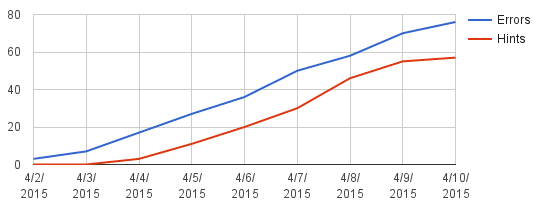
\includegraphics[width=1.0\columnwidth]{Body/figures/classoverflow/cumulativeErrorsAndHints.png}
\caption{Between Dear Beta's release (4/2) and the lab's due date (4/10), verification errors were consistently being entered into the system. The addition of hints followed close behind.}
\label{fig:betaengagement}
\end{figure}


\subsection{Dear Gamma Study}

With the Dear Gamma hints, six of the nine laboratory subjects were able to improve the optimality of their circuits within the hour that the study took place. Figure \ref{fig:gammaresults} illustrates the subjects' revisions. One student only needed one set of pointing hints. Five students successfully revised their circuits after one set of pointing and one set of teaching hints. Four students received a set of final bottom-out hints as well. Three of those four students ($S_2$, $S_5$, and $S_9$) were still unable to successfully revise their circuits. 

{\bf Hint Distribution} Figure \ref{fig:sankey} is a Sankey diagram of the optimization hints collected by Dear Gamma. The number of hints between certain key transitions, such as between the most common and the most optimal solutions, was far greater because of the lecturer's requests for pedagogically valuable hint prompts that introduced hint-writers to the common and optimal solutions. 

The most common solution size was 114 transistors. Students with that common solution were randomly assigned to generate hints from one of the many different larger solutions down to theirs. These hints are pooled together with the hints written by students with solutions larger than 114 transistors who are seeing the common 114-transistor solution for the first time. Less than five percent of students' solutions were the most optimal (96 transistors), but, at the request of the lecturer, every student was asked to consider that most optimal solution and write a hint for a fellow student on how to optimize their solution into that most optimal solution.

Students in the study were drawn from the same population as the hint-generating students, and all study subjects were offered the same number of hints (5 pointing hints, followed by 5 teaching hints, followed by 5 bottom-out hints) over the course of the hour-long session, regardless of the solution they started with. 

\begin{table*}[t]
  \begin{center}
    \begin{tabular}{|l|r|r|l|}
\hline
      {\bf Hint type} & {\bf Count} & {\bf (\%)} & {\bf Representative examples} \\
\hline
      Pointing ($p$) & 62 & 14\% & ``You don't have to keep S and Cout as two separate/independent CMOS gates.'' \\
      \hline
      Pointing and teaching ($pt$) & 81 & 19\% & ``Instead of making the S and Cout components individual, \\
& & & combine them together to save computation power.'' \\
\hline
      Teaching ($t$) & 111 & 26\% & ``Instead of recalculating values, save computation results to save time!'' \\
\hline
      Teaching and & 19 & 4\% & ``Via application of demorgan's theorem, \\
bottom-out ($tb$) & & & NAND2 (XOR A B) Cin is equivalent to NAND3(NAND2 A B) Cin.''\\
\hline
      Bottom-out ($b$) & 78 & 18\% & ``Use the output of a xor b for one of the nand2 gates.'' \\
\hline
      Unhelpful/irrelevant & 14 & 3\% & ``Use the hints provided by the lab, but try to improve on them.'' \\
\hline
No coder agreement & 70 & 16\% & \\
\hline
    \end{tabular}
 \caption{Breakdown of Dear Gamma hints by type. Students in the Dear Gamma lab study initially received 5 pointing hints ($p$), followed by 5 pure teaching hints ($t$), and finally 5 pure bottom-out hints ($b$), delivered whenever the student was stuck and asked for more help. }
 \label{tab:hintTypes}
  \end{center}
   
\end{table*}


{\bf Hint Types} Table \ref{tab:hintTypes} shows the breakdown of hints by type, along with representative examples. The Cohen's $\kappa$ \cite{cohen1960coefficient} inter-rater reliability was 0.54, which indicated that the two coders had moderate agreement across the six hint categories \cite{viera2005understanding}. 

{\bf Hint Prompt} Hint-authors interpreted the prompt to create a hint in different ways. Some addressed the hint-receiver directly ({\it ``Keep in mind that...''}), while others addressed the teaching staff ({\it ``I would mention [to the student]...''}). Some hint-authors did not directly write a hint, but instead wrote about how they would approach the situation of being a lab assistant for the hint-receiver: {\it ``I think first I'd ask to make sure they knew what a NAND3 was, because I think a solution like this might come from not totally understanding how it works.''} Still others took a conversational approach, as if they were having an unfolding conversation with the hint-receiver. Interestingly, a number of hint-authors referred to ``here'' or ``my circuit'' in their hints, as if the hint-receiver would be looking at the Dear Gamma interface, with all its examples, rather than just the text generated by the hint-author. This particular assumption on the part of the hint-author was confusing for hint-receivers.

{\bf Optimization Issues} $S_5$ was the only student who had a standard, optimizable solution, received hints, and had no insights about how to optimize the circuit within the allotted hour. $S_1$, $S_2$, and $S_9$'s forward progress was confounded by having near-optimal top-level architecture and very large (suboptimal) implementations of the underlying modules. Dear Gamma only shows hint-authors the top-level architecture, not the underlying gate implementations, for the alternative solutions they compare their own solutions to. They therefore found the hints, which were often about fixing high-level architecture, irrelevant and unhelpful. Even so, $S_1$ was still able to revisit the hints and correctly extract the lesson that only inverting gates should be used. As a result, $S_1$ successfully optimized their circuit.

While working through their optimizations and hints, $S_6$ was the one student who significantly deviated from the correct line of thought by removing all inverting gates.\footnote{Optimal solutions have {\it only} inverting gates.} As soon as $S_6$ saw that their transistor count had increased rather than decreased, they revisited the hints, realized their mistake, and correctly optimized their circuit. None of the hints themselves were incorrect, though some were deemed irrelevant or unhelpful.

{\bf Hint Progression} One student successfully optimized their solution from 150 transistors to the most common solution, 114 transistors, using only pointing and teaching hints. With some time left in the hour-long session, the student opted to optimize their circuit further. The experimenter gave the student one last set of hints, for the transition from 114 to the optimal 96-transistor solution. However, the experimenter did not restart the progression for this next transition; the student was given a set of bottom-out hints. Based on these hints, the student got the final optimization step without understanding, and appeared to feel cheated from the satisfaction of figuring it out himself. 

{\bf Student Reactions} The six subjects without suboptimal gates agreed with the statement {\it ``Overall, these hints helped me get to a more optimal circuit''} ($\mu$=6, $\sigma$=1.1 on a 7-point Likert scale). The remaining three subjects with suboptimal gates disagreed with the same statement ($\mu$=2.6, $\sigma$=2.1 on a 7-point Likert scale). Regardless of whether a subject's solution included suboptimal gates, subjects on average agreed with the statement {\it ``Hints helped me think differently about the problem, even if they didn't directly help me solve the problem'' } ($\mu$=5.4, $\sigma$=1.6).



\begin{figure}
\centering
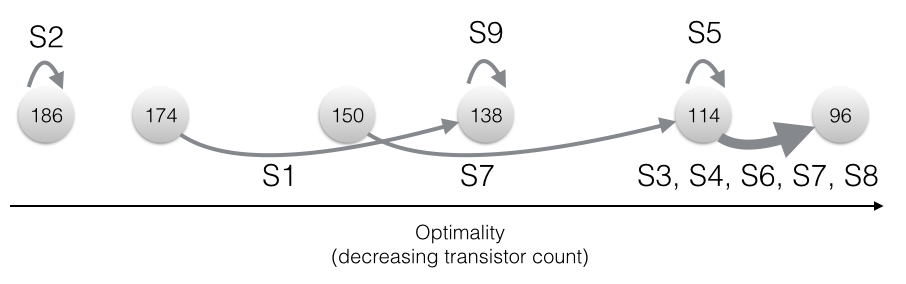
\includegraphics[width=1.0\columnwidth]{Body/figures/classoverflow/dearGammaResults.png}
\caption{Six of the nine lab study subjects were able to improve the optimality of their circuits with the help of the Dear Gamma hints. Subject S7 was able to make two leaps--one to a common solution with 114 transistors and another from the common solution to the most optimal solution at 96 transistors.}
\label{fig:gammaresults}
\end{figure}

Some subjects commented on the redundancy within each set of five hints of a particular type. This was sometimes expressed as a negative, as in {\it ``These are all hinting at the same thing but I want new information,''} and sometimes expressed as a positive, as in {\it ``Several hints are mentioning X.... I should look into it.''} One student told the experimenter that, while the individual hints were hard to understand, together they formed a clearer picture in her mind about what to do.


\section{Discussion}
In this section, we first address the research questions the evaluation was intended to answer. We then explain that, of the design decisions made during the design of Dear Beta and Dear Gamma, the critical factors for success included prompt clarity, the index chosen for hints, how alternative solutions are represented, and the use of hint progressions.

\subsection{Answers to Research Questions}

Our study sought to evaluate the characteristics of student-generated hints. We can see from Table \ref{tab:hintTypes} that students, without coaching, can naturally produce hints that point, teach, give a bottom-out direction, or provide some combination of those elements. However, the number of pointing hints labeled by {\it both} coders as purely pointing-type (22) was much smaller than the number of such hints in the teaching (75) and bottom-out (64) categories. Because students were not informed that their hint would be slotted into a progression, it is possible they may have felt that if they were going to give a future student one hint, it would need to be more substantial than just pointing to a particular location in the solution and hoping the hint-receiver would see the possibility of optimization.

Secondly, the studies sought to evaluate whether learners can solve problems using these hints. Both studies suggest that these student-written hints are helpful. The aggregate activity of students and teachers on Dear Beta indicate that the resource was populated with helpful hints. The Dear Gamma lab study was set up based on the observed sub-optimality of students' circuits at the level of choosing and arranging gates. Students whose solutions were suboptimal in that anticipated way rated the hints as helpful. Students whose solutions were suboptimal in unanticipated ways, i.e., at the level of the gates themselves, were not well-served by the hints. Future optimization hint workflows will need both (1) an optimality metric that accounts for multiple common types of suboptimality and (2) a representation of solutions with an appropriate level of detail about the difference between any two solutions. Regardless, the Dear Gamma study suggests that students are helped by the hints when the optimality metric and representation are appropriate.

\subsection{Lessons for Self-Reflection and Comparison Workflows}

Prompt clarity appears to be critical for soliciting the highest possible quality of hints from students. In Dear Gamma, hint collection and delivery were separate processes. Some students misunderstood the prompt and wrote hints as if their audience was still the teacher, not a fellow student. Others did not understand that the hint-receiver would only see the text of their hint, not the diagrams it was based on. In Dear Beta, hint collection and delivery were all mediated through the same, constantly updated interface. The appropriate audience for a hint was clear. Future instantiations of the self-reflection and comparison workflows should clarify who the audience is for hint-authors, perhaps by displaying what learners will see. 

The selection of an index for hints in the self-reflection workflow matters. In Dear Beta, the choice of test file name and test number as an index for hints worked well for a class of hundreds of students. In a MOOC-sized course, the index may need to include an indicator that specifies how the test failed as well. Indices in future systems should have sufficient information to group related hints into clusters of a manageable size.

The success of the comparison workflow depends not only on the index for solutions, but also on how these solutions are represented in the workflow's prompt for hints. In the comparison workflow, we found that transistor counts sometimes did not account for lower-level reasons for a suboptimal circuit, resulting in hints that were unhelpful for solutions with lower-level suboptimality. Students will not generate hints that account for what has been abstracted away in the representation of solutions in the hint prompt. Likewise, if the definition of optimality used to index solutions does not account for a certain kind of suboptimality, the hints generated will be unlikely to help future students with that kind of suboptimality. 

Lastly, when students request hints as they did in the Dear Gamma lab study, conforming to the intelligent tutoring system model of providing progressively specific hints is recommended. To automatically create hint progressions in the future, we could apply machine learning methods to estimate a given hint's type. Alternatively, we could learnersource hint classification. 

\subsection{Generalization}
Although we applied these workflows to computer architecture problems, the self-reflection and comparison workflows could be extended to other domains. The workflows can be most readily applied to solutions that can be objectively tested for satisfying a set of requirements, e.g., passing unit tests, or whose optimality can be objectively measured. In domains without objective test cases or definitions for optimality, it may be more difficult to establish indices for clustering hints. In these cases, students could be asked to write what challenge they overcame or select from a growing list, enabling others to search for those terms. The comparison workflow could be modified to simply pair students with solutions different than their own, letting them judge for themselves which they think is better, the alternative solution or their own, and write hints based on that judgment.

\todo{add this: "In the next academic year, we plan to expand our deployment of Dear Beta to two new classes: a MOOC version of the computer architecture class in this paper and a residential college-level software engineering course taken by several hundred students each term. Solutions in the software engineering course are written in Java and tested against teacher-designed test suites. Each error could be specified by the problem set number, test name, and line number. The implementation of Dear Beta has been written generally so that it can simultaneously support both classes, each with their own schema for describing an error."}

\section{Conclusions}
This paper enriches learnersourcing by shaping the design space for learnersourcing personalized hints, and presenting two workflows that engage learners in hint creation while reflecting on their own work as well as that of peers. We built Dear Beta and Dear Gamma, which apply these workflows to the creation of debugging and optimization hints, matching students to the appropriate hint creation task given their current progress. Results from our deployment study and subsequent lab study demonstrate the feasibility of these workflows, and indicate that learner-generated hints are helpful to learners. They also shed light on critical factors that may impact the quality of learnersourced hints, laying the groundwork for future systems in this area.